\subsection{Návrhové vzory}

Návrhový vzor je pojmenované a popsané řešení typického problému. Princip existují už dlouho: v architektuře -- např. barokní styl, literatura -- tragický hrdina, romantická novela\dots

V software se mnohé postupy \uv{vynalézají} stále znovu -- návrhové vzory mají potom pro typickou situaci popisovat:
\begin{pitemize}
	\item jak a kdy mají být objekty vytvářeny
	\item jaké vztahy a struktury mají obsahovat třídy
	\item jaké chování mají mít třídy, jak mají spolupracovat objekty
\end{pitemize}

Návrhový vzor (design pattern) je tedy obecně znovupoužitelné řešení problémů často se vyskytujících při návrhu softwaru. Nejedná se o hotový design, který by se dal transformovat přímo na kód -- je to víceméně jen popis nebo šablona, jak řešit nějaký problém vyskytující se ve více různých situacích. Objektově-orientované návrhové vzory typicky ukazují vztahy a interakce mezi třídami nebo objekty -- bez specifikace konkrétních konečných tříd nebo objektů. Algoritmy nejsou považovány za návrhové vzory, protože řeší spíše výpočetní problémy než designové.

Ne všechny softwarové vzory (software patterns) jsou návrhové. Návrhové vzory řeší problémy na úrovni návrhu softwaru (software desing). Jiné druhy vzorů (jako např. architekturální vzory (architectural patterns)) popisují problémy a řešení, které se zaměřují na jiné úrovně.

Základní prvky návrhových vzorů:
\begin{pitemize}
	\item \emph{Název} -- co nejvíce vystihující podstatu, usnadnění komunikace -- společný slovník
	\item \emph{Problém} -- obecná situace kterou má NV řešit
	\item \emph{Podmínky} -- popis okolností ovlivňujících použití NV a kontextu vhodném pro použití; některé okolnosti mohou být využity při řešení, jiné naopak jsou v konfliktu
	\item \emph{Řešení} -- soubor pravidel a vztahů popisujících jak dosáhnout řešení problému; nejen statická struktura, ale i dynamika chování
	\item \emph{Souvislosti a důsledky} -- detailní vysvětlení použití, implementace a principu fungování; způsob práce s NV v praxi
	\item \emph{Příklady} -- definice konkrétního problému, vstupní podmínky, popis implementace a výsledek
	\item \emph{Související vzory} -- použití jednoho NV nepředstavuje typicky ucelené řešení -- řetězec NV
\end{pitemize}

\ramcek{14.5cm}{
\emph{Nasledujúce sa vyučuje na predmete Návrhové vzory, ktorý je odporúčaný až pre nmgr štúdium}:\par
	Kategorie základních NV:
	\par\begin{center}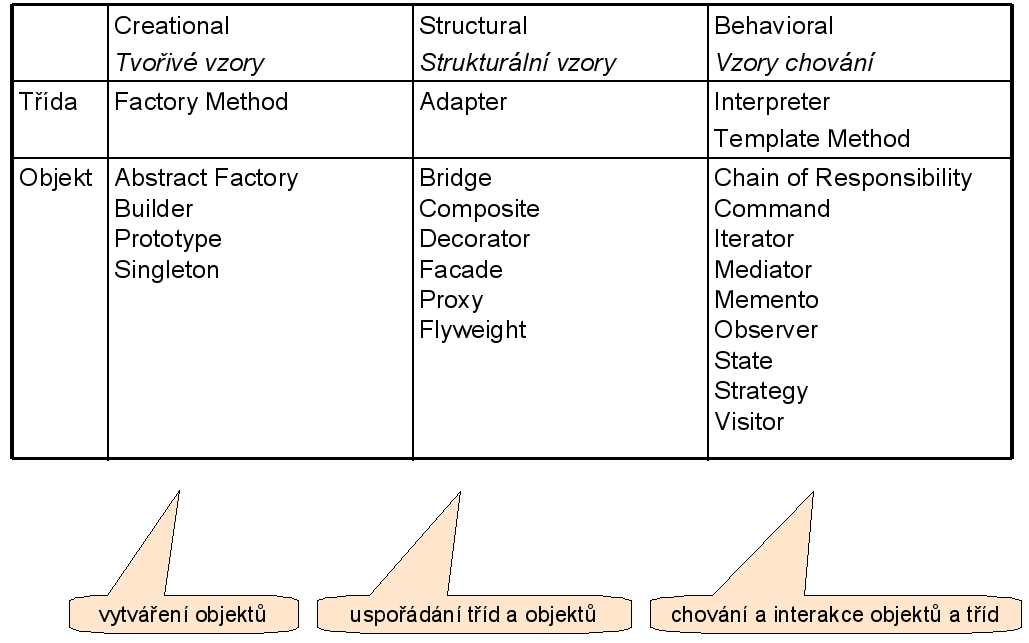
\includegraphics[width=12cm]{informatika/programovanie/obrazky/designpatterns.png}\end{center}
	
	Návrhové vzory je možno klasifikovat dle problémů které řeší. Príklady klasifikace vzorů podle řešených problémů:
	\begin{pitemize}
		\item \emph{Fundamental patterns}: ??? nevyhodíme to, je to jen na wiki a nepopsane
		\item \emph{Creation patterns}: vytváření objektů
		\item \emph{Structural patterns}: jak jsou třídy a objekty složený do větších struktur
		\item \emph{Behavioral patterns}: rozdělení funkčnosti a zodpovědnosti mezi objekty; komunikace mezi objekty; umožňuje zaměřit se při návrhu na propojení tříd, ne na běhové detaily
		\item \emph{Concurrency patterns} ??? tohle taky
	\end{pitemize}
}

\begin{priklady}
Creational patterns:
\begin{pitemize}
    \item Factory method (zajišťuje rozhodnutí o typu vytvářeného objektu při polymorfismu)
    \item Prototype (jak klonovat objekty)
    \item Singleton (jak omezit objekt jen na 1 instanci)
\end{pitemize}

Structural patterns:
\begin{pitemize}
    \item Adapter (konverze rozhraní objektů)
    \item Bridge (oddělení rozhraní a implementace třídy)
    \item Composite (jak složit více objektů do jednoho s jednotným přístupem)
    \item Proxy (jak zajistit přístup k jinému objektu přes můj objekt)
    \item Decorator (jak změnit vlastnosti třídy nebo zajistit rozšířenou funkčnost bez odděďování)
\end{pitemize}

Behavioral patterns:
\begin{pitemize}
    \item Chain of responsibility (jak určit kdo vykoná akci, když z venku přijde požadavek)
    \item Command (odstínění klienta od zpracování požadavku -- klient neurčuje kdy a jak se to provede)
    \item Iterator (projití prvků pole bez znalosti jejich implementace)
    \item Visitor (navštívení všech objektů nějaké struktury a práce s nimi, aby všechny nemusely implementovat stejné metody (a měnit se při jejich změně))
    \item Template (jak mohou odvozené třídy ovlivňovat algoritmy bázové třídy)
\end{pitemize}
\end{priklady}


TODO: rozšíriť, doplniť, opraviť :-)
